
\documentclass[aspectratio=169]{beamer}

% --- THEME AND STYLING ---
\usetheme{Madrid}
\useoutertheme{default}
\useinnertheme{rectangles}

% Remove navigation symbols for a clean look
\setbeamertemplate{navigation symbols}{}

% --- CUSTOM SKY-BLUE COLOR PALETTE ---
\definecolor{SkyBlue}{RGB}{135, 206, 235}  % Main theme color
\definecolor{DarkNavy}{RGB}{0, 0, 139}    % Contrast for titles and structure
\definecolor{LightBlueBg}{RGB}{240, 248, 255} % Very light blue for block bodies
\definecolor{AccentBlue}{RGB}{70, 130, 180}  % For alerted blocks
\definecolor{DarkGreyText}{RGB}{50, 50, 50}  % Body text color for readability
\definecolor{HighlightGreen}{RGB}{34, 139, 34}  % For positive highlights
\definecolor{AlertRed}{RGB}{220, 20, 60}  % For warnings

% --- APPLYING THE COLORS ---
\setbeamercolor{palette primary}{bg=SkyBlue,fg=DarkNavy}
\setbeamercolor{palette secondary}{bg=DarkNavy,fg=white}
\setbeamercolor{palette tertiary}{bg=AccentBlue,fg=white}
\setbeamercolor{palette quaternary}{bg=SkyBlue,fg=DarkNavy}

\setbeamercolor{structure}{fg=DarkNavy}
\setbeamercolor{section in toc}{fg=DarkNavy}
\setbeamercolor{subsection in head/foot}{bg=AccentBlue,fg=white}

\setbeamercolor{title}{fg=DarkNavy, bg=white}
\setbeamercolor{subtitle}{fg=DarkGreyText}
\setbeamercolor{author}{fg=DarkNavy}
\setbeamercolor{institute}{fg=DarkGreyText}
\setbeamercolor{date}{fg=DarkNavy}

\setbeamercolor{frametitle}{bg=SkyBlue,fg=DarkNavy}

\setbeamercolor{block title}{bg=DarkNavy,fg=white}
\setbeamercolor{block body}{bg=LightBlueBg,fg=DarkGreyText}
\setbeamercolor{block title alerted}{bg=AccentBlue,fg=white}
\setbeamercolor{block body alerted}{bg=LightBlueBg,fg=DarkGreyText}
\setbeamercolor{block title example}{bg=AccentBlue,fg=white}
\setbeamercolor{block body example}{bg=LightBlueBg,fg=DarkGreyText}

% Clean footer
\setbeamertemplate{headline}{}
\setbeamertemplate{footline}[frame number]
\setbeamercolor{footline}{fg=DarkNavy}

% Block appearance
\setbeamertemplate{blocks}[rounded][shadow=false]

% --- PACKAGES ---
\usepackage[utf8]{inputenc}
\usepackage{amsmath}
\usepackage{amssymb}
\usepackage{booktabs}
\usepackage{graphicx}
\usepackage{array}
\usepackage{multirow}
\usepackage{tikz}
\usetikzlibrary{shapes,arrows,positioning,calc,patterns}
\usepackage{siunitx}
\usepackage{textcomp}
\usepackage{enumitem}

% --- TITLE PAGE INFORMATION ---
\title[PVDF in Energy Storage]{Polyvinylidene Fluoride (PVDF) in Energy Storage}
\subtitle{From Incumbent Binder to Next-Generation Functional Material}
\author{CLL770 Final Presentation}
\institute{Department of Chemical Engineering}
\date{\today}% --- BEGIN DOCUMENT ---
\begin{document}

% --- TITLE SLIDE ---
\begin{frame}[plain]
    \titlepage
\end{frame}

% --- TABLE OF CONTENTS ---
\begin{frame}{Outline}
    \tableofcontents
\end{frame}

%%%%%%%%%%%%%%%%%%%%%%%%%%%%%%%%%%%%%%%%%%%%%%%%%%%%%%%%%%%%%%%%%
\section{Introduction \& Polymer Science}
%%%%%%%%%%%%%%%%%%%%%%%%%%%%%%%%%%%%%%%%%%%%%%%%%%%%%%%%%%%%%%%%%

\begin{frame}{What is Polyvinylidene Fluoride (PVDF)?}
    \begin{block}{A Critical Fluoropolymer}
        \begin{itemize}
            \item PVDF is a high-performance, semi-crystalline, thermoplastic fluoropolymer
            \item Synthesized from vinylidene fluoride (VDF) monomer: \textbf{-[CH$_2$-CF$_2$]-}$_n$
            \item Defining trait: \textbf{Highly polar C-F bonds} creating large dipole moment
            \item Unique property combination:
                \begin{itemize}
                    \item Exceptional chemical resistance
                    \item High thermal stability (stable $>$400\si{\celsius})
                    \item Inherent UV and weather resistance
                \end{itemize}
        \end{itemize}
    \end{block}
    
    \begin{alertblock}{Critical Role in Energy Storage}
        \textbf{Dual Function in Lithium-Ion Batteries:}
        \begin{enumerate}
            \item Industry-standard \textbf{polymeric binder} for electrode fabrication
            \item High-performance material for advanced \textbf{battery separators}
        \end{enumerate}
    \end{alertblock}
\end{frame}

\begin{frame}{Synthesis \& Molecular Weight}
    \begin{columns}[T]
        \begin{column}{0.55\textwidth}
            \begin{block}{Synthesis Process}
                \begin{itemize}
                    \item Free-radical polymerization of VDF monomer
                    \item Emulsion or suspension methods
                    \item Control over molecular weight (MW) and distribution
                    \item Critical manufacturing parameter for end-use
                \end{itemize}
            \end{block}
            
            \begin{alertblock}{Why MW Matters for Batteries}
                \begin{itemize}
                    \item \textbf{High Molecular Weight grades required} for binder applications
                    \item Long polymer chains create more entanglement points
                    \item Provides strong adhesion and mechanical cohesion
                    \item Essential for holding electrode particles together
                \end{itemize}
            \end{alertblock}
        \end{column}
        
        \begin{column}{0.4\textwidth}
            \begin{center}
                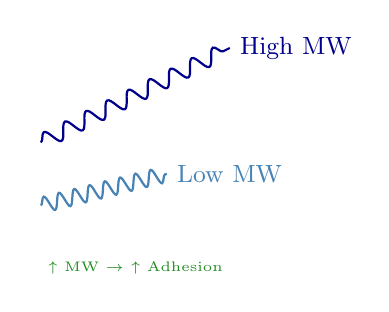
\begin{tikzpicture}[scale=0.8]
                    % Polymer chain representation
                    \draw[thick, DarkNavy, decorate, decoration={snake, amplitude=1mm, segment length=3mm}] 
                        (0,0) -- (3,1.5) node[right, font=\small] {High MW};
                    \draw[thick, AccentBlue, decorate, decoration={snake, amplitude=1mm, segment length=2mm}] 
                        (0,-1) -- (2,-0.5) node[right, font=\small] {Low MW};
                    
                    % Properties
                    \node[font=\tiny, text width=2.5cm, align=center] at (1.5,-2) 
                        {\textcolor{HighlightGreen}{$\uparrow$ MW $\rightarrow$ $\uparrow$ Adhesion}};
                \end{tikzpicture}
            \end{center}
        \end{column}
    \end{columns}
\end{frame}
        \begin{itemize}
            \item **High Molecular Weight (MW) grades are required** for binder applications.
            \item \textbf{Reason:} The long polymer chains create a greater number of entanglement points and van der Waals interactions.
            \item \textbf{Result:} This provides the strong adhesion and mechanical cohesion needed to hold the electrode together.
        \end{itemize}
    \end{alertblock}
\end{frame}

\begin{frame}{The Key to PVDF: Crystalline Polymorphism}
    \begin{columns}[T] % T = align at top
        \begin{column}{0.5\textwidth}
            [cite_start]\begin{block}{$\alpha$-Phase (Alpha) [cite: 23-25]}
                \begin{itemize}
                    \item The most common and thermodynamically stable phase.
                    \item Forms when PVDF crystallizes from a melt.
                    \item \textbf{Conformation:} Trans-Gauche-Trans-Gauche' (TGTG').
                    \item \textbf{Property:} Dipoles cancel out, making the phase **non-polar** and non-piezoelectric.
                \end{itemize}
            \end{block}
        \end{column}
        
        \begin{column}{0.5\textwidth}
            [cite_start]\begin{alertblock}{$\beta$-Phase (Beta) [cite: 26-30]}
                \begin{itemize}
                    \item The most technologically significant phase.
                    \item Forms via mechanical stretching or **solution-casting** (using polar solvents).
                    \item \textbf{Conformation:} All-Trans (TTTT).
                    \item \textbf{Property:} All C-F dipoles align, creating a massive net dipole moment. This makes the phase **highly polar** and piezoelectric.
                \end{itemize}
            \end{alertblock}
        \end{column}
    \end{columns}
    
    [cite_start]\begin{exampleblock}{The Processing-Phase-Property Link [cite: 31, 38]}
        The choice of manufacturing (e.g., solvent) can create functionally different materials from the same polymer.
        \begin{itemize}
            [cite_start]\item One study found a **$\beta$-dominant PVDF binder** yielded a battery with much higher discharge capacity (\SI{185}{mAh/g}) and superior capacity retention (98\% vs 71.6\%) compared to an $\alpha$-phase sample[cite: 38].
        \end{itemize}
    \end{exampleblock}
\end{frame}

%%%%%%%%%%%%%%%%%%%%%%%%%%%%%%%%%%%%%%%%%%%%%%%%%%%%%%%%%%%%%%%%%
\section{Quantified Properties for Batteries}
%%%%%%%%%%%%%%%%%%%%%%%%%%%%%%%%%%%%%%%%%%%%%%%%%%%%%%%%%%%%%%%%%

\begin{frame}{Key Thermal Properties}
    \begin{columns}[T]
        \begin{column}{0.5\textwidth}
            [cite_start]\begin{block}{Glass Transition Temp ($T_g$) [cite: 45, 47, 48]}
                \begin{itemize}
                    \item \textbf{Value:} \SIrange{-35}{-40}{\celsius}.
                    \item \textbf{Significance:} This is far below the battery's operating temperature.
                    \item \textbf{Result:} The binder's amorphous regions are in a **rubbery, flexible state**. This imparts toughness and allows the binder to accommodate small volume changes (e.g., in graphite) without cracking.
                \end{itemize}
            \end{block}
        \end{column}
        
        \begin{column}{0.5\textwidth}
            [cite_start]\begin{alertblock}{Melting Temp ($T_m$) [cite: 51, 54-56]}
                \begin{itemize}
                    \item \textbf{Value:} \SIrange{165}{175}{\celsius}.
                    \item \textbf{Significance:} This is a critical safety advantage, especially for separators.
                    \item \textbf{Result:} Standard polyolefin (PE/PP) separators melt at \SI{\sim 130}{\celsius}. PVDF's higher $T_m$ provides a **"higher safety margin"** and prevents catastrophic internal short circuits during overheating.
                \end{itemize}
            \end{alertblock}
        \end{column}
    \end{columns}
\end{frame}

\begin{frame}{Stability \& The "Master Property"}
    [cite_start]\begin{block}{Thermal Stability (Decomposition) [cite: 63, 65, 66]}
        \begin{itemize}
            \item \textbf{Value:} PVDF is exceptionally stable, with an onset of decomposition **above \SI{400}{\celsius}**.
            \item \textbf{Significance:} Electrodes are dried at \SI{\sim 130}{\celsius} to evaporate the NMP solvent.
            \item \textbf{Result:} This provides an exceptionally wide and safe processing window, ensuring the polymer's integrity is maintained during manufacturing.
        \end{itemize}
    \end{block}

    [cite_start]\begin{exampleblock}{Percent Crystallinity (\%) — The "Master Property" [cite: 58, 59]}
        \begin{itemize}
            \item \textbf{Value:} Typical grades are 50-70% crystalline, but battery grades are specifically manufactured with a wide range (e.g., 14% to 32%).
            \item \textbf{Significance:} This property must be carefully optimized to **balance mechanical strength, adhesion, and electrolyte uptake**.
        \end{itemize}
    \end{exampleblock}
\end{frame}

\begin{frame}{The Critical Crystallinity Trade-Off: Data}
    [cite_start]\frametitle{The Critical Crystallinity Trade-Off: Data [cite: 89]}
    \begin{table}
        [cite_start]\caption{Influence of PVDF Binder Crystallinity on Electrode Properties (Data from [cite: 3, 89])}
        \centering
        \small % Make table text smaller
        \begin{tabular}{l c c l}
            \toprule
            \textbf{Property} & \textbf{PVDF 1 (Low)} & \textbf{PVDF 2 (High)} & \textbf{Key Takeaway} \\
            \midrule
            \% Crystallinity & 14\% & 32\% & Input Variable \\
            \textbf{Adhesion Strength} & 1.30 N-cm⁻¹ & \textbf{11.42 N-cm⁻¹} & \textbf{High crystallinity = 9x higher adhesion} \\
            \textbf{Electrolyte Uptake} & \textbf{18.88\%} & 11.3\% & Low crystallinity = more swelling \\
            \midrule
            \textbf{Capacity Retention} & 64\% (500 cycles) & \textbf{82\% (500 cycles)} & \textbf{High adhesion & low swelling wins} \\
            \bottomrule
        \end{tabular}
    \end{table}
\end{frame}

\begin{frame}{The Critical Crystallinity Trade-Off: Analysis}
    [cite_start]\frametitle{The Critical Crystallinity Trade-Off: Analysis [cite: 91-98]}
    
    [cite_start]\begin{block}{Crystallinity $\rightarrow$ Adhesion [cite: 91]}
        The high-crystallinity binder (PVDF 2) has **~9x stronger adhesion**. This is due to "higher intermolecular interaction between PVDF polymer chains."
    \end{block}
    
    [cite_start]\begin{block}{Crystallinity $\rightarrow$ Swelling [cite: 92, 93]}
        The low-crystallinity binder (PVDF 1) has a much larger amorphous volume, which is the only region the electrolyte can penetrate. This leads to **significantly higher electrolyte uptake (swelling)**.
    \end{block}
    
    [cite_start]\begin{alertblock}{The Non-Obvious Conclusion [cite: 95-97]}
        The high-crystallinity (low swelling) binder performed *better*.
        \begin{itemize}
            \item \textbf{Why?} **Excessive swelling is detrimental**.
            \item The high swelling of PVDF 1 "destructs the distribution of conducting carbon in the electrode," which increases internal resistance and leads to rapid capacity fade.
            \item \textbf{Goal:} Optimize crystallinity to be high enough for adhesion, but low enough for *controlled* swelling.
        \end{itemize}
    \end{alertblock>
\end{frame}

\begin{frame}{Electrochemical & Chemical Properties}
    \begin{columns}[T]
        \begin{column}{0.5\textwidth}
            [cite_start]\begin{block}{Electrochemical Stability [cite: 101, 104]}
                \begin{itemize}
                    \item \textbf{The "Gold Standard":} PVDF is stable within a wide \textbf{0-5 V window}.
                    \item \textbf{Significance:} It is one of the few polymers stable at both the low-potential graphite anode (\SI{\sim 0.1}{V}) and high-voltage cathodes (>\SI{4.3}{V}).
                \end{itemize}
            \end{block}
            
            [cite_start]\begin{block}{Dielectric Constant ($\epsilon$) [cite: 107, 111-113]}
                \begin{itemize}
                    \item \textbf{Value:} High (\(\epsilon\) = 8.4 to 12).
                    \item \textbf{Significance:} A major advantage for separators. The high polarity "ensures easy wetting" and aids in dissociating lithium salts, which promotes higher ionic conductivity.
                \end{itemize}
            </block}
        \end{column}
        
        \begin{column}{0.5\textwidth}
            [cite_start]\begin{alertblock}{Solubility: The NMP Link [cite: 120, 124-128]}
                \begin{itemize}
                    \item \textbf{Property:} PVDF has very limited solubility, dissolving only in strong polar aprotic solvents (NMP, DMF, DMSO).
                    \item \textbf{Industry Standard:} N-methyl-2-pyrrolidone (NMP) is used due to its high flash point and recyclability.
                    \item \textbf{The Crisis:} NMP is classified as a **Substance of Very High Concern (SVHC)** and a reproductive hazard, creating immense regulatory and cost pressure to find alternatives.
                \end{itemize}
            \end{alertblock}
        </column>
    \end{columns}
\end{frame}

%%%%%%%%%%%%%%%%%%%%%%%%%%%%%%%%%%%%%%%%%%%%%%%%%%%%%%%%%%%%%%%%%
\section{Advanced Characterization Methods}
%%%%%%%%%%%%%%%%%%%%%%%%%%%%%%%%%%%%%%%%%%%%%%%%%%%%%%%%%%%%%%%%%

\begin{frame}{How Properties Are Measured (I)}
    \begin{columns}[T]
        \begin{column}{0.5\textwidth}
            \begin{block}{Phase & Crystallinity}
                \begin{itemize}
                    [cite_start]\item \textbf{FTIR:} Identifies the crystal phase ($\alpha$ vs. $\beta$) by measuring specific "vibrational fingerprints" (e.g., $\beta$-phase peak at \SI{838}{cm^{-1}})[cite: 151, 157].
                    [cite_start]\item \textbf{XRD:} Quantifies the *degree* of crystallinity by integrating the area under the sharp crystalline peaks relative to the broad amorphous "halo"[cite: 159, 161].
                \end{itemize}
            \end{block}
        \end{column}
        
        \begin{column}{0.5\textwidth}
            \begin{block}{Thermal Analysis}
                \begin{itemize}
                    \item \textbf{DSC (Calorimetry):} Measures heat flow to find key transitions. [cite_start]It reveals the $T_g$ as a small "step" and the $T_m$ as a large "peak" [cite: 169-172].
                    \item \textbf{TGA (Gravimetric):} Measures sample mass as it is heated. [cite_start]It confirms the decomposition temperature (e.g., stable up to >\SI{400}{\celsius})[cite: 176, 178].
                \end{itemize}
            \end{block}
        \end{column}
    \end{columns}
    
    \vfill
    [cite_start]\placeholder{Insert Example: DSC/TGA Thermogram [cite: 174, 178]}
    
\end{frame}

\begin{frame}{How Properties Are Measured (II)}
    [cite_start]\begin{block}{Slurry Rheology (Flow) [cite: 181, 187-191]}
        \begin{itemize}
            \item \textbf{Tool:} Rotational Rheometer.
            \item \textbf{Why:} "Processability" is critical. The slurry must be viable for high-speed industrial coating.
            \item \textbf{Required Behaviors:}
                \begin{enumerate}
                    \item \textbf{Shear-Thinning:} Viscosity decreases at high shear (during coating).
                    \item \textbf{Viscoelastic (Gel-like):} Stable solid at rest ($G' > G''$) to prevent heavy particles from settling.
                \end{enumerate}
        \end{itemize}
    \end{block}
    
    \begin{columns}[T]
        \begin{column}{0.5\textwidth}
            [cite_start]\begin{block}{Mechanical Analysis [cite: 195, 198]}
                \begin{itemize}
                    \item \textbf{Tool:} Peel Test.
                    \item \textbf{What:} Quantifies "adhesion strength."
                    \item \textbf{How:} A machine pulls the electrode coating off the foil and records the force required (in N/cm).
                \end{itemize}
            \end{block}
        \end{column}
        \begin{column}{0.5\textwidth}
            [cite_start]\begin{block}{Electrochemical Analysis [cite: 200-205]}
                \begin{itemize}
                    \item \textbf{Tool:} EIS (Impedance Spectroscopy).
                    \item \textbf{What:} Measures ionic conductivity of swollen PVDF.
                    \item \textbf{How:} Probes the stability of the binder-electrode interface over time (degradation appears as an increase in resistance).
                \end{itemize}
            \end{block}
        \end{column}
    \end{columns}
\end{frame}

%%%%%%%%%%%%%%%%%%%%%%%%%%%%%%%%%%%%%%%%%%%%%%%%%%%%%%%%%%%%%%%%%
\section{Application Deep Dive: Binders \& Separators}
%%%%%%%%%%%%%%%%%%%%%%%%%%%%%%%%%%%%%%%%%%%%%%%%%%%%%%%%%%%%%%%%%

\begin{frame}{Application I: The Electrode Binder}
    [cite_start]\begin{block}{Primary Role: Cohesion & Adhesion [cite: 209, 211]}
        Despite being only 2-5\% of the electrode's weight, its function is non-negotiable. It acts as a polymeric "glue" with two mechanical functions:
        \begin{itemize}
            \item \textbf{Cohesion:} Binds active material particles (e.g., NCM) and conductive carbon additives to each other.
            \item \textbf{Adhesion:} Adheres this entire composite matrix to the metal current collector (aluminum or copper foil).
        \end{itemize}
    \end{block}
    
    [cite_start]\begin{block}{Electrochemical Requirements [cite: 220-223]}
        To function, the binder must satisfy three conditions:
        \begin{enumerate}
            \item \textbf{Electrochemical Stability:} Must be inert in the 0-5 V window.
            \item \textbf{Chemical Inertness:} Must not react with the electrolyte.
            \item \textbf{Controlled Swelling:} Must absorb electrolyte to create an ion-conductive pathway, but not swell so much that it destroys the electrode's conductive network.
        \end{enumerate}
    \end{block}
\end{frame}

\begin{frame}{A Fundamental Limitation: The Silicon Anode}
    [cite_start]\begin{alertblock}{The Problem with Silicon [cite: 228, 229]}
        \begin{itemize}
            \item Silicon (Si) is the most promising next-gen anode, offering \textbf{10x the theoretical capacity} of graphite.
            \item \textbf{The Catch:} It experiences massive, destructive **volume expansion of over 300\%** during charging (lithiation).
        \end{itemize}
    \end{alertblock}
    
    [cite_start]\begin{block}{PVDF's Failure [cite: 230-233]}
        \begin{itemize}
            \item The mechanical properties of PVDF (high modulus) make it too **stiff and brittle** to accommodate this extreme strain.
            \item The "rigid PVDF shell" cannot stretch; it simply **"cracks."**
            \item This leads to the "pulverization" of the electrode, a complete loss of electrical contact, and rapid, irreversible battery failure.
        \end{itemize}
    \end{block>
    
    \vfill
    \placeholder{Insert Infographic:
    Graphite (small expansion) vs. Silicon ( >300\% expansion)
    [cite_start][cite: 1, 229]}
    
\end{frame}

\begin{frame}{Application II: The High-Performance Separator}
    [cite_start]\frametitle{Application II: The High-Performance Separator [cite: 236-240]}
    
    \begin{block}{Dual Functions}
        \begin{enumerate}
            \item \textbf{Physical Separation:} Acts as a physical barrier to prevent the anode and cathode from touching (which would cause a short circuit).
            \item \textbf{Ionic Transport:} Its microporous structure is filled with liquid electrolyte, allowing Li$^+$ ions to pass through freely.
        \end{enumerate}
    \end{block}
    
    \begin{alertblock}{The Quantitative Advantage vs. Polyolefins (PE/PP)}
        PVDF separators are a premium, high-safety alternative. A quantitative comparison reveals why:
        \begin{itemize}
            \item \textbf{Safety (Melting Temp):} PVDF melts at \SI{\sim 170}{\celsius}, far higher than PE at \SI{\sim 130}{\celsius}. [cite_start]This provides a crucial safety margin against thermal runaway[cite: 242].
            \item \textbf{Performance (Wettability):} PVDF's high polarity gives it "excellent wettability" with polar electrolytes. [cite_start]This lowers internal resistance and allows for "faster charging"[cite: 242, 245].
            [cite_start]\item \textbf{Capacity (Uptake):} PVDF can hold significantly more electrolyte (92-95\% uptake vs. 48-65\% for PE/PP)[cite: 242, 243].
        \end{itemize}
    \end{alertblock}
\end{frame}

\begin{frame}{Table: Separator Material Comparison}
    [cite_start]\frametitle{Quantitative Separator Comparison [cite: 242, 243]}
    \begin{table}
        \centering
        \small
        \caption{Comparative Analysis of Battery Separator Materials}
        \begin{tabular}{l l l l}
            \toprule
            \textbf{Property} & \textbf{Standard PE/PP Separator} & \textbf{PVDF Separator} & \textbf{Benefit} \\
            \midrule
            [cite_start]\textbf{Melting Temp ($T_m$)} & \SIrange{\sim 130}{165}{\celsius} & \textbf{\SI{\sim 170}{\celsius}} & \textbf{Higher safety margin} [cite: 242] \\
            [cite_start]\textbf{Wettability} & Poor (non-polar) & \textbf{Excellent (highly polar)} & Lower resistance, faster charging [cite: 242] \\
            [cite_start]\textbf{Electrolyte Uptake} & 48\% - 65\% & \textbf{92\% - 95\%} & Higher ion-carrying capacity [cite: 242, 243] \\
            [cite_start]\textbf{Fabrication} & Limited (stretching) & \textbf{Tunable (Electrospinning)} & Optimized pore structure [cite: 243] \\
            \bottomrule
        \end{tabular}
    \end{table}
\end{frame}

%%%%%%%%%%%%%%%%%%%%%%%%%%%%%%%%%%%%%%%%%%%%%%%%%%%%%%%%%%%%%%%%%
\section{Sustainability Crisis \& Alternatives}
%%%%%%%%%%%%%%%%%%%%%%%%%%%%%%%%%%%%%%%%%%%%%%%%%%%%%%%%%%%%%%%%%

\begin{frame}{The Sustainability Crisis (I): The NMP Problem}
    [cite_start]\frametitle{The Sustainability Crisis (I): The NMP Problem [cite: 251, 253]}
    
    [cite_start]\begin{alertblock}{Toxicity and Regulation [cite: 255]}
        \begin{itemize}
            \item The industrial reliance on N-methyl-2-pyrrolidone (NMP) is PVDF's primary liability.
            \item NMP is not just toxic; it is classified as a **"Substance of Very High Concern (SVHC)"** by the European Chemicals Agency (ECHA).
            \item It is a known **reproductive toxicant** ("may damage the unborn child").
            \item Its use is now heavily restricted by regulations like EU REACH, driving up compliance costs.
        \end{itemize}
    \end{alertblock}
    
    [cite_start]\begin{block}{Cost: The "Aqueous Processing Revolution" [cite: 257-260]}
        \begin{itemize}
            \item Water as a solvent: < \$0.02 / Liter.
            \item NMP as a solvent: \$1.00 - \$3.00 / Liter (\textbf{50-150x more expensive}).
            \item Furthermore, NMP processing requires a massive, high-energy, high-capital-cost **solvent recovery infrastructure**, which is not required for water.
        \end{itemize}
    \end{block}
\end{frame}

\begin{frame}{The Sustainability Crisis (II): End-of-Life Recycling}
    [cite_start]\frametitle{The Sustainability Crisis (II): End-of-Life Recycling [cite: 262]}
    \begin{columns}[T]
        \begin{column}{0.5\textwidth}
            [cite_start]\begin{alertblock}{Pyrometallurgy (Burning) [cite: 264-268]}
                \begin{itemize}
                    \item \textbf{Process:} High-temp incineration to recover metals.
                    \item \textbf{The Problem:} When PVDF is burned, it decomposes and releases large quantities of **highly corrosive and toxic Hydrogen Fluoride (HF) gas**.
                    \item \textbf{Impact:} This poses a severe health risk, requires costly "acid scrubbers," and can even deactivate the valuable cathode materials being recovered.
                \end{itemize}
            </end{alertblock}
        \end{column}
        
        \begin{column}{0.5\textwidth}
            [cite_start]\begin{block}{Hydrometallurgy (Leaching) [cite: 269-271]}
                \begin{itemize}
                    \item \textbf{Process:} Uses acids to dissolve and separate metals.
                    \item \textbf{The Problem:} PVDF's "exceptional chemical resistance" means it **does not dissolve**.
                    \item \textbf{Impact:} It remains as a solid contaminant, complicating the separation and purification of the valuable metal salts.
                \end{itemize}
            </{block}
        \end{column}
    \end{columns}
\end{frame}

\begin{frame}{Alternative Binders: The Aqueous Revolution}
    [cite_start]\frametitle{Alternative Binders: The Aqueous Revolution [cite: 284, 296-300]}
    
    \begin{block}{Challenging a Misconception: Adhesion}
        \begin{itemize}
            \item A common assumption is that PVDF has superior adhesion.
            [cite_start]\item \textbf{The Data Contradicts This:} Quantitative tests show that major aqueous binders (PAA, CMC, Alginate) exhibit \textbf{stronger adhesion} than PVDF[cite: 296, 297].
        \end{itemize}
    \end{block}
    
    \begin{exampleblock}{The Reason: Hydrogen Bonding}
        \begin{itemize}
            [cite_start]\item Aqueous binders (like PAA and CMC) are rich in carboxyl (\textbf{-COOH}) and hydroxyl (\textbf{-OH}) functional groups[cite: 298].
            [cite_start]\item These groups form strong, high-energy **hydrogen bonds** with the oxide layers on the active materials and current collector[cite: 299].
            [cite_start]\item PVDF lacks these groups and relies on weaker, non-specific van der Waals forces[cite: 300].
        \end{itemize}
    \end{exampleblock}
    
    \vfill
    \placeholder{Insert Infographic:
    Chemical Structures of PVDF vs. PAA/CMC
    (Illustrating H-Bonding sites) [cite_start][cite: 1, 298]}
    
\end{frame}

\begin{frame}{Quantitative Binder Comparison}
    [cite_start]\frametitle{Quantitative Binder Comparison [cite: 292, 293]}
    \begin{table}
        \centering
        \small
        \caption{Quantitative Comparison of Battery Binder Properties}
        \begin{tabular}{l l l l l}
            \toprule
            \textbf{Polymer Property} & \textbf{PVDF (Incumbent)} & \textbf{PAA (Si-Anode)} & \textbf{CMC (Aqueous)} & \textbf{Alginate (Aqueous)} \\
            \midrule
            [cite_start]\textbf{Processing Solvent} & \textbf{NMP (Toxic)} & \textbf{Water} & \textbf{Water} & \textbf{Water} [cite: 292] \\
            [cite_start]\textbf{Adhesion (N/cm)} & \(\sim\)1.0 & \(\sim\)1.5 & 1.1 - 1.7 & \textbf{\(\sim\)2.0} [cite: 292] \\
            [cite_start]\textbf{Modulus (MPa)} & 600-4000 & \textbf{\(\sim\)8000} & 1000 & 119-500 [cite: 292] \\
            [cite_start]\textbf{$T_g$ (Flexibility)} & \SI{-35}{\celsius} (Flexible) & \SI{\sim 106}{\celsius} (Elastic) & \SI{186}{\celsius} (Rigid) & --- [cite: 293] \\
            \bottomrule
        \end{tabular}
    \end{table}
    
    [cite_start]\begin{alertblock}{Analysis: The Right Binder for the Job [cite: 302, 329]}
        \begin{itemize}
            \item The table shows PVDF is mechanically outclassed for specific roles.
            [cite_start]\item \textbf{For Silicon Anodes:} PVDF fails[cite: 329]. [cite_start]**PAA is the binder of choice** due to its unique combination of high stiffness (\SI{\sim 8000}{MPa}) and elasticity, allowing it to withstand the high mechanical stresses of Si expansion[cite: 302].
        \end{itemize}
    \end{alertblock}
\end{frame}

%%%%%%%%%%%%%%%%%%%%%%%%%%%%%%%%%%%%%%%%%%%%%%%%%%%%%%%%%%%%%%%%%
\section{The Future of PVDF \& Market Analysis}
%%%%%%%%%%%%%%%%%%%%%%%%%%%%%%%%%%%%%%%%%%%%%%%%%%%%%%%%%%%%%%%%%

\begin{frame}{The Future of PVDF: Evolving Its Role}
    [cite_start]\frametitle{The Future of PVDF: Evolving Its Role [cite: 343]}
    
    \begin{columns}[T]
        \begin{column}{0.5\textwidth}
            [cite_start]\begin{block}{Gel-Polymer Electrolytes (GPEs) [cite: 345, 350-352]}
                \begin{itemize}
                    \item PVDF-HFP copolymers are ideal hosts for GPEs.
                    \item The polymer matrix swells, trapping liquid electrolyte to form a "gel."
                    \item \textbf{Result:} A flexible, non-leaking "solid" that retains the high ionic conductivity of a liquid (\SI{e-4} to \SI{e-3}{S/cm}).
                \end{itemize}
            \end{block}
        \end{column}
        
        \begin{column}{0.5\textwidth}
            [cite_start]\begin{exampleblock}{Composite Solid-State Electrolytes (SSEs) [cite: 357-361]}
                \begin{itemize}
                    \item Purely ceramic SSEs are brittle and have poor electrode contact.
                    \item \textbf{Solution:} Use PVDF as a **flexible polymer matrix** to host the ceramic particles.
                    \item \textbf{Result:} This solves the mechanical and interfacial problems, creating a flexible, high-performance solid-state electrolyte.
                \end{itemize}
            </exampleblock>
        \end{column}
    \end{columns}
\end{frame}

\begin{frame}{A New Incompatibility: Sodium-Ion Batteries (SIBs)}
    [cite_start]\frametitle{A New Incompatibility: Sodium-Ion Batteries (SIBs) [cite: 363, 364]}
    
    \begin{block}{The Problem}
        PVDF's success in LIBs does \textbf{not} translate to SIBs. It is **fundamentally electrochemically unstable** in a sodium-based system.
    \end{block}
    
    [cite_start]\begin{alertblock}{The Failure Mechanism [cite: 366-370]}
        \begin{enumerate}
            \item During sodium insertion (sodiation), PVDF undergoes a chemical decomposition reaction.
            \item This reaction produces fluoride ions (F⁻).
            \item These fluoride ions react with sodium to form a stable, insulating \textbf{"NaF layer"} (sodium fluoride) on the electrode surface.
            \item This resistive layer causes the binder to lose its ability to bind effectively, leading to high resistance and rapid cell failure.
        \end{enumerate}
    \end{alertblock>
\end{frame}

\begin{frame}{Market \& Techno-Economic Analysis}
    \begin{columns}[T]
        \begin{column}{0.5\textwidth}
            [cite_start]\begin{block}{Market Size & Growth [cite: 373-386]}
                \begin{itemize}
                    \item Driven by EV and grid storage sectors.
                    \item \textbf{2024 Value:} US\$ 5.99 Billion.
                    \item \textbf{2033 Forecast:} US\$ 28.75 Billion.
                    \item \textbf{CAGR:} 20.3\%.
                    \item \textbf{Key Players:} Arkema (Kynar®), Solvay/Syensqo (Solef®), Kureha.
                    \item \textbf{Geography:} APAC region is dominant (56.67\% share) due to China's manufacturing.
                \end{itemize}
            \end{block}
        \end{column}
        
        \begin{column}{0.5\textwidth}
            [cite_start]\begin{alertblock}{The *Real* Cost Problem [cite: 405-416]}
                The polymer itself is not the main cost (industrial price: \$\SIrange{7}{26}{/kg}).
                \vspace{0.3cm}
                The \textbf{Total Cost of Ownership} is the problem:
                \begin{enumerate}
                    \item \textbf{Solvent Cost:} NMP is 50-150x more expensive than water.
                    \item \textbf{CAPEX:} Massive capital cost for high-energy NMP recovery systems.
                    \item \textbf{OPEX:} High energy cost to dry the high-boiling-point NMP.
                    \item \textbf{Compliance Cost:} Meeting environmental \& health laws.
                \end{enumerate}
            </end{alertblock}
        \end{column}
    \end{columns}
\end{frame}

%%%%%%%%%%%%%%%%%%%%%%%%%%%%%%%%%%%%%%%%%%%%%%%%%%%%%%%%%%%%%%%%%
\section{Conclusions \& Future Outlook}
%%%%%%%%%%%%%%%%%%%%%%%%%%%%%%%%%%%%%%%%%%%%%%%%%%%%%%%%%%%%%%%%%

\begin{frame}{Conclusion: The PVDF Paradox}
    [cite_start]\frametitle{Conclusion: The PVDF Paradox [cite: 419]}
    
    \begin{columns}[T]
        \begin{column}{0.5\textwidth}
            [cite_start]\begin{block}{The Entrenched Incumbent [cite: 421-423]}
                \begin{itemize}
                    \item \textbf{Unmatched Stability:} Its 0-5 V electrochemical window is uniquely suited for high-voltage cathodes that power the EV revolution.
                    \item \textbf{Ideal Processing:} Its rheological behavior in NMP is the backbone of efficient, large-scale industrial manufacturing.
                \end{itemize}
            \end{block}
        \end{column}
        
        \begin{column}{0.5\textwidth}
            [cite_start]\begin{alertblock}{The Fatal Flaws [cite: 424-429]}
                \begin{itemize}
                    \item \textbf{Processing:} Relies on the toxic, stringently regulated, and expensive NMP solvent.
                    \item \textbf{Recycling:} Creates hazardous Hydrogen Fluoride (HF) gas when burned.
                    \item \textbf{Next-Gen Anodes:} Mechanically incompatible (too brittle) for high-capacity silicon anodes.
                    \item \textbf{Next-Gen Chemistries:} Chemically incompatible with sodium-ion batteries (forms NaF).
                \end{itemize}
            </alertblock}
        </{column}
    \end{columns}
\end{frame}

\begin{frame}{Future Research Outlook}
    [cite_start]\frametitle{Future Research Outlook [cite: 431-443]}
    
    \begin{block}{Path 1: "Greening" PVDF}
        \begin{itemize}
            \item Preserve PVDF's performance while eliminating NMP.
            \item Focus on validating and scaling up \textbf{"green solvent"} processing (e.g., DMSO, DMI).
            \item Pair with "direct recycling" processes to dissolve and recover PVDF and cathodes intact.
        \end{itemize}
    \end{block}
    
    \begin{block}{Path 2: "Replacing" PVDF}
        \begin{itemize}
            \item Accept PVDF's limitations and focus on functional replacements.
            \item Design functional polymers (like PAA) that offer \textbf{superior adhesion} and the mechanical flexibility to \textbf{"unlock" silicon anodes}.
        \end{itemize}
    \end{block}
    
    \begin{block}{Path 3: "Evolving" PVDF}
        \begin{itemize}
            \item Leverage PVDF's unique polarity and swelling for new applications.
            \item Use as a sophisticated polymer matrix for \textbf{Gel-Polymer (GPEs)} and \textbf{Composite Solid-State (SSEs)} batteries.
        \end{itemize}
    \end{block>
\end{frame}

\begin{frame}{References}
    \begin{block}{Source Material}
        All content presented is derived from the provided research report:
        
        \vspace{0.5cm}
        \textit{"Polyvinylidene Fluoride (PVDF) in Energy Storage: A Critical Review of Polymer Properties, Application Performance, and Market Dynamics in Lithium-Ion Batteries and Beyond"}
        
        \vspace{0.5cm}
        All citations (e.g.,) refer to the works cited list within that source document.
    \end{block}
\end{frame}


% --- FINAL SLIDE ---
\begin{frame}[plain]
    \vfill
    \begin{center}
        {\Huge \textcolor{DarkNavy}{Thank You}}
        
        \vspace{1cm}
        
        {\Large Questions and Discussion}
    \end{center}
    \vfill
\end{frame}

\end{document}